% This is LLNCS.DEM the demonstration file of
% the LaTeX macro package from Springer-Verlag
% for Lecture Notes in Computer Science,
% version 2.4 for LaTeX2e as of 16. April 2010
%
\documentclass{llncs}
%
\usepackage{makeidx}  % allows for indexgeneration
\usepackage{llncsdoc}
\usepackage{algorithmic}
\usepackage{amssymb}
\usepackage{graphicx}
\usepackage{wrapfig}
\usepackage{cite}
\usepackage{amsmath}
\usepackage[usenames,dvipsnames]{xcolor}
\usepackage[parfill]{parskip} 

\newcommand{\Mod}[1]{\ (\text{mod}\ #1)}
\newcommand{\todo}[1]{{\color{red}{TODO #1}}}
\renewcommand\refname{Referin\c{t}e}
\setcounter{secnumdepth}{4}

%
\begin{document}
\pagestyle{empty}
%
%
\title{TODO}
%
\titlerunning{Research report for UROP course}  % abbreviated title (for running head)
%                                     also used for the TOC unless
%                                     \toctitle is used
%
\subtitle{Undergraduate Research Opportunities}
\author{Drago\c{s} Alin Rotaru}
\authorrunning{D.A.Rotaru} % abbreviated author list (for running head)
%
%%%% list of authors for the TOC (use if author list has to be modified)
%\tocauthor{}

\institute{Universitatea din Bucuresti, Romania\\
\email{r.dragos0@gmail.com
}
}


\maketitle              % typeset the title of the contribution

\begin{abstract}
  None
\keywords{securitate, scheme de partajare}
\end{abstract}

%----------------------------------------------------------------
%----------------------------------------------------------------
%----------------------------------------------------------------
%----------------------------------------------------------------
%----------------------------------------------------------------

\section{Introducere}
\label{sec:intro}

\subsection{Istoric}
Termenul de criptografie este definit in dictionarul Oxford ca fiind "arta de a scrie si a rezolva coduri".
Criptografia moderna s-a desprins de cea clasica in jurul anilor '80, motivand implementarea rigurozitatii matematice pentru definirea constructiilor criptografice. Asta pentru ca in anii anteriori, experienta a dovedit nesiguranta metodelor de criptare, criptanaliza lor fiind uneori triviala (cifrul lui Cezar, Vigenere \ref{wiki:caesar}, \ref{wiki:vigenere}) sau uneori atinsa cu ceva mai mult efort precum Enigma si alte metode din cel de-al doilea razboi mondial. \ref{wiki:enigma}

Criptografia moderna se gaseste pretutindeni in viata de zi cu zi de la ATM-uri, cartele telefonice la semnaturi digitale, protocoale de autentificare, licitatii electronice sau bani digitali, luand amploare o data cu aparitia sistemelor cu cheie publica. O definitie potrivita ar fi "studiul stiintific al tehnicililor pentru a securiza informatia digitala, tranzactiile si calculul distribuit.". \cite{Katz:2007}

\subsection{Motivatie}
\todo{nu are leg\u{a}tur\u{a}: faptul ca sunt scheme cuantice nu are impact asupra structurii de acces; e ok sa men\c{t}ionezi, dar atunci faci asta \^{i}n sec\c{t}iunea anterioar\u{a}, c\^{a}nd po\c{t}i s\u{a} adaugi \c{s}i alte modalit\u{a}\c{t}i de definire: scheme bazate pe latici, scheme bazate pe perechi biliniare, scheme cuantice, etc.}
%TODO: maybe wrap this up in a definition
Dezavantajul schemelor generale de partajare este dimensiunea componentelor, exponentiala in functie de numarul de participanti. \cite{Survey:2011}
De asemenea, s-au dezvoltat scheme pentru modele de calcul neconventional, cum ar fi cel cuantic. \cite{hillery:1999} %maybe expand this
%Poate aici vine mai bine sub sectiunea cu securitatea teoretica

\subsection{Structura}
TODO

%----------------------------------------------------------------
%---------------------------------------------------------------
%----------------------------------------------------------------
%----------------------------------------------------------------
%----------------------------------------------------------------

\subsection{Securitatea Teoretica a Informatiei}

In cazul unor criptosisteme acestea nu pot fi compromise chiar daca adversarul dispune de o putere computationala nelimitata. Cateva exemple de criptosisteme care garanteaza securitatea teoretica-informationala sunt: schemele de partajare, unele protocoale multi-party computation, preluarea intr-un mod sigur(securizat?) informatii de la baze de date. Securitatea teoretica vine insa cu un cost: efortul computational depus este mult mai mare decat in cazul schemelor care nu garanteaza securitatea teoretica (se bazeaza pe dificultatea computationala unor probleme cunoscute). \cite{L:1997}

%----------------------------------------------------------------
%----------------------------------------------------------------
%----------------------------------------------------------------
%----------------------------------------------------------------
%----------------------------------------------------------------
\section{Scheme de partajare}

\label{sec:encryption}
%TODO: find translation for multi party computation

O schem\u{a} de partajare const\u{a} \^{i}n distribuirea unei informa\c{t}ii secrete $\mathcal{S}$ la mai mul\c{t}i participan\c{t}i $\mathcal{P} = \{P_1, \dots, P_n\}$ astfel \^{i}nc\^{a}t oricare mul\c{t}ime de participan\c{t}i predefinit\u{a}  ca f\u{a}c\^{a}nd parte dintr-o structur\u{a} de acces pe care o vom denumi $\mathcal{A}$ s\u{a} poat\u{a} reconstitui secretul $\mathcal{S}$.
Formal, o schem\u{a} de partajare este reprezentat\u{a} de o pereche de algoritmi \textbf{$(Gen, Rec)$}:
\begin{itemize}
	\item \textit{$Gen(S, m)$} este un algoritm care prime\c{s}te la intrare un secret \textit{S} \c{s}i un num\u{a}r \^{i}ntreg $m$ \c{s}i \^{i}ntoarce un set de componente ${s_1, s_2, \dots, s_m}$.
	\item \textit{$Rec({s_i}_1, {s_i}_2, \dots, {s_i}_q)$} este un algoritm care prime\c{s}te ca parametri de intrare o mul\c{t}ime de componente \c{s}i \^{i}ntoarce \textit{S} dac\u{a} mul\c{t}imea $\{{P_i}_1, {P_i}_2, \dots, {P_i}_q \} \in \mathcal{A}$.
\end{itemize} 
%todo: add some more text between itemizers
Majoritatea schemelor constau \^{i}n mai multe etape precum:
\begin{itemize}
	\item \textit{Ini\c{t}ializare}. Presupune ini\c{t}ializarea variabilelor de mediu necesare.
	\item \textit{Generare}. O entitate autorizat\u{a} (numit\u{a} dealer) $\mathcal{D}$ folose\c{s}te algoritmul \textit{Gen} pentru a genera componentele.
	\item \textit{Distribu\c{t}ie}. Componentele sunt trimise participan\c{t}ilor cu ajutorul unui mijloc de comunicare sigur, f\u{a}r\u{a} ca acestea sa fie vizibile unui atacator.
	\item \textit{Reconstruc\c{t}ie}. D\^{a}ndu-se o mul\c{t}ime de componente, se folose\c{s}te algoritmul \textit{Rec} pentru a recupera secretul
	$\mathcal{S}$.
\end{itemize}

Schemele de partajare se clasific\u{a} in func\c{t}ie de cantitatea de informa\c{t}ie secret\u{a} pe care o pot ob\c{t}ine persoanele care nu fac parte din $\mathcal{A}$ \cite{Martin:2008}:
\begin{itemize}
	\item \textit{Sisteme perfecte de partajare}: componentele nu ofer\u{a} nici o informatie teoretic\u{a} despre $\mathcal{S}$ indiferent de resursele computa\c{t}ionale.
	\item \textit{Sisteme statistic sigure}: o frac\c{t}iune de informa\c{t}ie este dezvaluit\u{a} despre $\mathcal{S}$ independent de puterea computional\u{a} a adversarului.
	\item \textit{Sisteme computa\c{t}ional-sigure de partajare}: se bazeaz\u{a} pe faptul ca reconstituirea lui $\mathcal{S}$ se reduce la o problema \textit{dificil\u{a}} (spre exemplu problema Diffie-Hellman \cite{boneh:1998decision} ) \^{i}n lipsa unor informa\c{t}ii oferite doar grupului de acces $\mathcal{A}$.
%cite somehow AA article \todo{nu toate problemele sunt demonstrate ca fiind NP complete, se crede ca sunt probleme dificile}. ups, forgot about that:)
\end{itemize} 

\^{I}n continuare vom prezenta cateva sisteme perfecte de partajare utilizate \^{i}n cadrul unor arhitecturi pentru stocarea fisierelor pe o durata indelungat\u{a}.

\subsection{Istoric}

Primele scheme de partajare au fost dezvoltate independent de Shamir \c{s}i Blakley in 1979 \cite{B:1979, S:1979}.

Denumite \c{s}i scheme majoritare $(k, n)$, acestea rezolvau cazul \^{i}n care oricare grup de participan\c{t}i cu un num\u{a}r mai mare sau egal dec\^{a}t $k$  (m\u{a}rimea pragului) poate reconstitui secretul $\mathcal{S}$ din componentele primite de la dealer. Dac\u{a} schema este perfect \textit{sigur\u{a}} atunci oricare grup cu un num\u{a}r de participan\c{t}i mai mic decat $k$ nu ob\c{t}ine vreo informa\c{t}ie despre $\mathcal{S}$.

%Not\u{a}m $P = \{P_1, \dots, P_n\}$ mul\c{t}imea format\u{a} din cei $n$ participan\c{t}i \^{i}ntr-o schem\u{a} \c{s}i $y \leftarrow^R Y$ ca $y$ este un element ales uniform aleator din mul\c{t}imea $Y$.

Schemele majoritare (spre exemplu schema Shamir) sunt insuficiente pentru a permite partajarea pentru anumite structuri de acces. Consider\u{a}m cazul \^{i}n care vrem sa partajam un secret \^{i}ntre 4 participan\c{t}i: $P_1, P_2, P_3, P_4$ astfel \^{i}nc\^{a}t $\{P_1,P_2\}$ \c{s}i $\{P_3,P_4\}$ s\u{a} fie singurele mul\c{t}imi autorizate pentru reconstruc\c{t}ia secretului $S$ (i.e. $\mathcal{A} = \{ \{P_1,P_2\}, \{P_3,P_4\} \}$). \^{I}n mod evident, problema nu poate fi rezolvat\u{a} cu o structur\u{a} de acces de tip prag: anumite mul\c{t}imi de 2 participan\c{t}i trebuie s\u{a} poat\u{a} reconstrui secretul ($ \{P_1,P_2\}, \{P_3,P_4\} $), \^{i}n timp ce altele nu $( \{P_1,P_3\}, \{P_1,P_4\}, \{P_2,P_3\}, \{P_2,P_4\} $)

Astfel de scheme de partajare pentru structuri de acces generale au fost dezvoltate de Ito, Saito \c{s}i Nishizeki, realiz\^{a}nd o generalizare a schemei Shamir \cite{ITO:1989}.
Benaloh \c{s}i Leichter au demonstrat ca schemele de partajare de tip prag nu pot fi folosite pe structuri general monotone (familie de submul\c{t}imi ale lui $\mathcal{P}$ cu proprietatea c\u{a} dac\u{a} $A \in \mathcal{A}$ \c{s}i $A \subset A'$, atunci $A' \in \mathcal{A}$) \c{s}i ob\c{t}in o construc\c{t}ie mai eficient\u{a} ca Ito et. al din punct de vedere al num\u{a}rului de componente distribuite participan\c{t}ilor \cite{JJ:1990}.


\subsection{Schema unanim\u{a}}

Presupun\^{a}nd ca vrem s\u{a} imp\u{a}r\c{t}im un secret $\mathcal{S}$ la $n$ participan\c{t}i astfel \^{i}nc\^{a}t $\mathcal{S}$ sa poat\u{a} fi recuperat doar daca to\c{t}i cei $n$ participan\c{t}i \^{i}\c{s}i combin\u{a} componentele pe care le de\c{t}in. Metoda este echivalent\u{a} cu o schem\u{a} $(n, n)$ majoritar\u{a}. Un exemplu este schema introdus\u{a} de Karin, Greene \c{s}i Hellman (Fig.\ref{fig:all_or_nothing})  \cite{Karnin:83}.


%---------------- Figure - all_or_nothing - START ------------------------
\begin{figure*}[h!]

\begin{tabular}{|p{\textwidth}|}
\hline

\\
\hspace{.1in}
\textbf{Ini\c{t}ializare}: 
	\begin{itemize}
		\item Fie $S \in Z_q$ unde $q > 1 $ \c{s}i $q$ prim;
		\item Fie $n$ num\u{a}rul de participan\c{t}i;
	\end{itemize}
\medskip

\hspace{.1in}
\textbf{Generare}: Dealerul $\mathcal{D}$:
	\begin{itemize}
		\setlength{\itemsep}{5pt}
		\item Alege $n - 1$ valori aleatoare $s_i \leftarrow^R Z_p$, $i \in \{1,2,\dots,{n-1}\}$;
		\item $s_n = S + \sum\limits_{i=1}^{n-1} s_i \Mod q $;
	\end{itemize}
\medskip

\hspace{.1in}
\textbf{Distribu\c{t}ie}: Dealerul $\mathcal{D}$:
	\begin{itemize}
		\item transmite \^{i}n mod sigur participantului $P_i$ componenta $s_i$, $i \in \{1,2,\dots,n\}$;
	\end{itemize}

\hspace{.1in}
\textbf{Reconstruc\c{t}ie}: Cei $n$ participan\c{t}i:
	\begin{itemize}
		\item Calculeaz\u{a} $S = \sum\limits_{i=1}^{n} s_i \Mod q$.
	\end{itemize}

\\
\hline
\end{tabular}
\caption{Schema unanim\u{a} \cite{Karnin:83}}
\label{fig:all_or_nothing}
\end{figure*}

%---------------- Figure - all_or_nothing- STOP ------------------------



\subsection{Schema Shamir}
%TODO complete description

Schema Shamir ofer\u{a} mai mult\u{a} flexibilitate dec\^{a}t schema unanima prin faptul ca oricare $k$ (sau mai multi) participan\c{t}i
din cei $n$ pot recupera $\mathcal{S}$, \^{i}ns\u{a} mai pu\c{t}in de $k$ participan\c{t}i nu ob\c{t}in nicio informa\c{t}ie despre $\mathcal{S}$. Schema Shamir este deci o schem\u{a} $(k,n)$ majoritar\u{a}.

Intuitiv, av\^{a}nd $k$ puncte in plan $(x_i, y_i)$, $x_i \neq x_j \text{ } i,j \in \{1,2,\dots,k\}$ $\forall i \neq j$, exist\^{a} o curb\u{a} polinomial\u{a} unic\u{a} care trece prin ele.  
\^{I}n schimb, pentru a defini o curb\u{a} polinomial\u{a} de grad $k$ care trece prin $k - 1$ puncte date, exist\u{a} o infinitate de solu\c{t}ii.
Evident, orice submul\c{t}ime de valori $s_i$ de m\u{a}rime egal\u{a} cu $k$ este suficient\u{a} \c{s}i necesar\u{a} pentru a reconstrui polinomul $f$. Dupa interpolarea componentelor de\c{t}inute de cel pu\c{t}in $k$ dintre participan\c{t}i, secretul $\mathcal{S}$ se determin\u{a} ca fiind $f(0)$ (Fig. \ref{fig:shamir_scheme}) \cite{S:1979}.

Pentru un atacator care de\c{t}ine chiar \c{s}i $k-1$ valori $s_i$, acesta nu determin\u{a} nimic despre $\mathcal{S}$, spa\c{t}iul de solu\c{t}ii posibile fiind identic fa\c{t}\u{a} de situa\c{t}ia \^{i}n care nu reu\c{s}e\c{s}te sa ob\c{t}in\u{a} vreo component\u{a}.

%---------------- Figure - shamir_scheme - START ------------------------
\begin{figure*}[h!]

\begin{tabular}{|p{\textwidth}|}
\hline

\\
\hspace{.1in}
\textbf{Ini\c{t}ializare}: 
	\begin{itemize}
		\item Fie $S \in Z_q$ unde $q > 1 $ \c{s}i $q$ prim;
		\item Fie $n$ num\u{a}rul de participan\c{t}i a.i $q > n$;
		\item Fie $k$ num\u{a}rul minim de componente puse in comun pentru a determina pe $\mathcal{S}$;
	\end{itemize}
\medskip

\hspace{.1in}
\textbf{Generare}: Dealerul $\mathcal{D}$:
	\begin{itemize}
		\item Alege $n$ valori distincte $x_i \leftarrow^R Z_q \text{, }i = 1,2,\dots,n$;
		\item Alege $a_{i} \leftarrow^R Z_q \text{, }i \in \{1,2,\dots,{k - 1}$\}, $a_{k-1} \neq 0$;
		\item Construie\c{s}te polinomul $f(x) = a_{k - 1}x ^ {k-1} + a_{k-2}x ^ {k - 2} + \dots + a_1x + \mathcal{S}$;
		\item Calculeaz\u{a} $s_i = f(x_i) \text{ }, i \in \{1,2,\dots,n\}$;
	\end{itemize}
\medskip

\hspace{.1in}
\textbf{Distribu\c{t}ie}: Dealerul $\mathcal{D}$:
	\begin{itemize}
		\item Transmite participantului $P_i$ componenta $s_i$, $i \in \{1,\dots,n-1\}$;
	\end{itemize}

\hspace{.1in}
%TODO: aranjeaza cu "(sau mai mare)"
\textbf{Reconstruc\c{t}ie}: Orice mul\c{t}ime cu dimensiunea $k$ (sau mai mare) de participan\c{t}i distinc\c{t}i $P_1, P_2, \dots, P_k$:
	\begin{itemize}
		\setlength{\itemsep}{5pt}
		\item Interpoleaz\u{a} punctele $s_i$ pentru a ob\c{t}ine polinomul $f$:
		\begin{equation} f(x)=\sum_{i=1}^{k} {s_i}\prod_{1 \leq j \leq k, j \neq i} \frac{x-x_j}{x_i-x_j} \end{equation}
		\item Afl\u{a} secretul reconstruit $S = f(0)$.
	\end{itemize}

\\
\hline
\end{tabular}

\caption{Schema Shamir \cite{S:1979}}
\label{fig:shamir_scheme}
\end{figure*}

%---------------- Figure - shamir_scheme- STOP ------------------------

\subsection{Schema Ito, Saito \c{s}i Nishizeki}
\label{Ito}

\^{I}n continuare vom descrie modalitatea de distribuire a componentelor de la care au pornit Ito, Saito \c{s}i Nishizeki pentru ca schema sa aiba o structur\u{a} de acces $\mathcal{A} \subseteq 2^P$ (submul\c{t}ime a setului de participan\c{t}i) monotona (i.e. $\forall A \in \mathcal{A}, A \subseteq A' \Rightarrow A' \in \mathcal{A}$).
Folosind construc\c{t}ia unei scheme majoritare $(k, n)$ autorii au reu\c{s}it s\u{a} descrie elementele din $\mathcal{A}$ folosind rezultatul unei reuniuni de mul\c{t}imi de componente cu un num\u{a}r de elemente mai mare sau egal decat $k$ ( Fig. \ref{fig:ito_et_al}) \cite{ITO:1989}. Nota\c{t}ia $x : Pr$, \^{i}nseamn\u{a} c\u{a} $x$ are proprietatea $Pr$. 

Dezvantajul acestei structuri este num\u{a}rul de componente necesar pentru o structur\u{a} de acces oarecare $\mathcal{A}$. Un mod simplu de construire al func\c{t}iei $Assign$ este Pentru mai multe informatii despre functia $Assign$, cititorul interesat poate citi in \cite{ITO:1989}.
\todo{prezentarea trebuie s\u{a} fie de sine st\u{a}t\u{a}toare, trebuie m\u{a}car s\u{a} explici \^{i}n cuvinte ce \^{i}nseamn\u{a}}



%---------------- Figure - Ito_et_al- START ------------------------
\begin{figure*}[h!]

\begin{tabular}{|p{\textwidth}|}
\hline

\\
\hspace{.1in}
\textbf{Ini\c{t}ializare}: 
	\begin{itemize}
		\item Fie $q$ un num\u{a}r prim $q$, $q > 1$, $z \in \mathbb{N}$ nenul \c{s}i $\mathcal{C} = GF(p^z)$;
		\item Fie $S \in \mathcal{C}$ secretul; 
		\item Fie structura de acces $\mathcal{A}$;
		\item Fie $n$ num\u{a}rul de participan\c{t}i;
	\end{itemize}

\medskip

\hspace{.1in}
\textbf{Generare}: Dealerul $\mathcal{D}$:
	\begin{itemize}
		\setlength{\itemsep}{5pt}
		\item Alege $n$ valori distincte $x_i \leftarrow^R Z_q \text{, }i = 1,2,\dots,n$;
		\item Alege $a_{i} \leftarrow^R \mathcal{C} \setminus \{0\} \text{, }i \in \{1,2,\dots,{k - 1}\}$, $a_{k-1} \neq 0$;
		\item Construie\c{s}te polinomul $f(x) = a_{k - 1}x ^ {k-1} + a_{k-2}x ^ {k - 2} + .... + a_1x + \mathcal{S}$;
		\item Atribuie $s_i = f(x_i) \text{ } i \in \{1,2,\dots,n\}$; Fie $Shares = \{ s_1, \dots, s_n \}$;
		\item Alege $D_i \subseteq Shares \text{ } 1 \leq i \leq n$;
		\item Alege func\c{t}ia $Assign: P \rightarrow 2^Q$:
			\begin{itemize}
				\item $Assign(P_i) = D_i \text{ } 1 \leq i \leq n$
				\item $\mathcal{A} = \bigg \{ \ Q \subseteq Shares: \bigg| \underset{P_i \in Q}{{\bigcup}} Assign(P_i) \bigg| \geq k \bigg \}$;
				% : <=> having property
			\end{itemize}
	\end{itemize}
\medskip

\hspace{.1in}
\textbf{Distribu\c{t}ie}: Dealerul $\mathcal{D}$:
	\begin{itemize}
		\item Transmite participantului $P_i$ componenta $Assign(P_i)$, $i \in 1,2,\dots,n$;
	\end{itemize}

\hspace{.1in}
\textbf{Reconstruc\c{t}ie}: Participan\c{t}ii din structura de acces $\mathcal{A}$:
	\begin{itemize}
		\item Procedeaza identic ca in schema Shamir.
	\end{itemize}


\\
\hline
\end{tabular}

\caption{Schema Ito, Saito, si Nishizeki \cite{ITO:1989}}
\label{fig:ito_et_al}
\end{figure*}

%---------------- Figure - Ito_et_al - STOP ------------------------

%----------------------------------------------------------------
%----------------------------------------------------------------
%----------------------------------------------------------------
%----------------------------------------------------------------
%----------------------------------------------------------------



\section{Sisteme de stocare de lunga durata}

%TODO: key management issues
In acesta sectiune vom arata cateva intrebuintari ale schemelor de partajare. Consideram cazul in care vrem sa stocham rapoarte medicale, imagini, documente clasificate pe un timp indelungat intr-un mediu electronic. Pe parcursul timpului, pot apare in schimb, diverse probleme precum dezastre naturale, defectiunea unor componente hardware, eroare umana, etc. \cite{SGMV:2009}
Un sistem de stocare necesar nevoilor noastre trebuie sa satisfaca cel putin urmatoarele 3 conditii:
\begin{itemize}
	\item Disponibilitatea: Informatia trebuie sa ramana accesibila tot timpul, in ciuda erorilor de tip hardware.
	\item Integritatea: Abilitatea sistemului de a raspunde cererilor intr-un mod care garanteaza corectitudinea lor.
	\item Confidentialitatea: O persoana care nu face parte din grupul de acces sa nu obtina permisiunea de a afla informatii de orice fel despre datele existente in sistem.
\end{itemize}

\subsection{Criptare VS scheme de partajare}


Una dintre solutiile existente pentru a construi acest sistem ar putea fi criptarea datelor folosind o cheie inainte de inserarea lor in spatiul de stocare. In momentul in care un user autorizat doreste sa efectueze o citire a unor date, intrebuinteaza cheia potrivita pentru a le decripta.
In practica exista algoritmi de criptare eficienti precum AES ins\u{a} acea\c{s}tia nu garanteaz\u{a} confiden\c{t}ialitatea datelor \^{i}n cazul \^{i}n care avem de a face cu un adversar fara o limita computationala. Un dezavantaj al criptarii este adminstrarea cheilor, standardele de securitatea schimbandu-se in fiecare an.
De fiecare data cand cheile sunt inlocuite atunci este necesara recriptarea datelor de pe fiecare baza de date. Cu cat disponibilitatea este mai mare - numarul de noduri duplicate creste- recriptarea lor devine o operatie costisitoare. 

Majoritatea tehnicilor de criptarea se bazeaza pe dificultatea factorizarii unui numar sau cea a calcularii logaritmului discret insa o data cu posibila dezvoltare a calculatoarelor cuantice aceste probleme nu vor mai fi atat de dificile. \cite{Shor:1994}
----------------------------------------------------------------
%----------------------------------------------------------------
%----------------------------------------------------------------
%----------------------------------------------------------------
%----------------------------------------------------------------



\section{Sisteme de stocare de lung\u{a} durat\u{a} bazate pe scheme de partajare}

O alternativ\u{a} la solu\c{t}ia cu criptare care asigur\u{a} at\^{a}t confiden\c{t}ialitate c\^{a}t \c{s}i redundan\c{t}a necesar\u{a} este intrebuin\c{t}area sistemelor de stocare de lung\u{a} durat\u{a} bazate pe scheme de partajare. \cite{W:2000,SB:2005,SGMV:2009}

%Poate cateva detalii despre RAID
%Maybe some pictures with PASIS, just in case not enough pages

\subsection{PASIS}
\label{sec:desc_pasis}
PASIS este o solu\c{t}ie pentru un sistem descentralizat care ofer\u{a} beneficii precum securitate, redundan\c{t}\u{a} a datelor si auto-\^{i}ntre\c{t}inere.
Structurile descentralizate \^{i}mpart informa\c{t}ia la mai multe noduri folosind scheme de redundan\c{t}a precum RAID \todo{(R... A... I... D...) - mereu trebuie in paranteza denumirea completa, o singura data, cand se introduce o abreviere} pentru a asigura performan\c{t}a, scalabilitatea sistemului dar \c{s}i integritatea datelor. \cite{Patterson:1988}
\todo{exact, cateva detalii despre RAID}

PASIS folose\c{s}te schemele de partajare pentru a distribui informa\c{t}ia nodurilor de stocare dintr-o re\c{t}ea. Aceasta introduce agen\c{t}i pe partea clientului pentru a scrie sau \c{s}terge date din noduri, dar \c{s}i agen\c{t}i pentru mentenan\c{t}\u{a}. Componentele obt\c{i}nute \todo{\^{i}n urma partaj\u{a}rii unui} fisier sunt \todo{nu puse, ci stocate} in re\c{t}ea cu ajutorul agen\c{t}ilor (Fig. \ref{fig:pasis}). Pe l\^{a}ng\u{a} con\c{t}inutul brut al componentelor se adaug\u{a} metadate pentru a re\c{t}ine adresa nodului din re\c{t}ea la care au fost \todo{stocate, nu trimise} dar \c{s}i noua denumire cu care este salvat\u{a} in re\c{t}ea.

Consider\^{a}nd o schem\u{a} de partajare majoritar\u{a} $p-m-n$ unde oricare din cei $m$ participan\c{t}i pot reconstitui fisierul, dar mai pu\c{t}in de $p$ nu ob\c{t}in nicio informa\c{t}ie dintr-un total de $n$ componente. 
\todo{o schema de partajare majoritara are 2 parametrii, care sunt aici?! rescriere! aten\c{t}ie, s\u{a} folose\c{s}ti nota\c{t}iile de mai \^{i}nainte: n = nr de participan\c{t}i, etc.}

Atunci c\^{a}nd un participant ini\c{t}iaz\u{a} o cerere pentru a citi un fisier, agentul PASIS aflat local procedeaz\u{a} dupa cum urmeaz\u{a}:
\begin{itemize}
	\item Caut\u{a} numele celor $n$ componente care alc\u{a}tuiesc fi\c{s}ierul \^{i}ntr-un serviciu care listeaz\u{a} toate datele.
	\item Ini\c{t}iaza cereri de citire la cel pu\c{t}in $m$ din cele $n$ noduri.
	\item \^{I}n caz ca acesta nu prime\c{s}te cel pu\c{t}in $m$ r\u{a}spunsuri se intoarce la pasul anterior \^{i}ncerc\^{a}nd interog\u{a}ri la noduri diferite.
	\item Reconstituie fi\c{s}ierul ob\c{t}inut din cele $m$ componente.
\end{itemize}
Opera\c{t}ia de scriere este similar\u{a} cu cea de citire, aceasta oprindu-se atunci c\^{a}nd \^{i}n cel pu\c{t}in $n - m + 1$ noduri s-au stocat cu succes componente.
In articol se men\c{t}ioneaza \c{s}i compromisul de spa\c{t}iu-timp \todo{denumirea consacrat\u{a} \^{i}n romana este compromis spa\c{t}iu-timp, nu timp-spa\c{t}iu} folosite de PASIS \todo{: extinde pu\c{t}in ce \^{i}nseamn\u{a} asta}.
Autorii specific\u{a} solu\c{t}ii pentru auto mentenan\c{t}a sistemului cu ajutorul resurselor umane prin monitorizarea periodic\u{a} st\u{a}rii sistemului folosind log-uri sau ajustarea parametrilor din cadrul schemei de partajare.

\todo{Imi place figura! Dar citeaza lucrarea - \c{s}i in caption \c{s}i in text - nu am vazut nicio citare la PASIS!}

\begin{figure}
	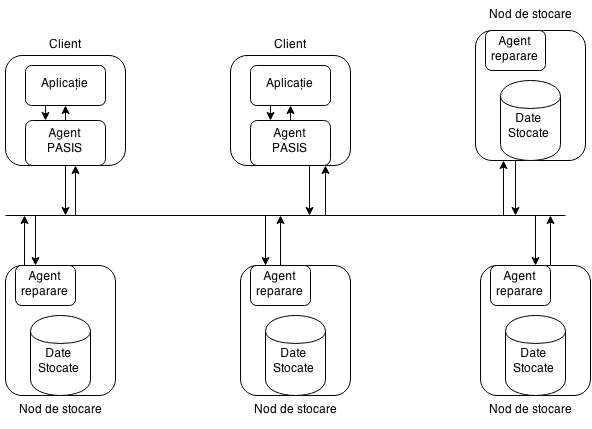
\includegraphics[width=11cm]{img/PASIS.png}
	\caption{Arhitectura PASIS cu $4$ noduri \c{s}i $2$ clien\c{t}i \cite{}}
	\label{fig:pasis}
	\bigskip
\end{figure}

\subsection{GridSharing} 
\^{I}n 2005, Subbiah \c{s}i Blough propun o nou\u{a} abordare pentru a construi un sistem de stocare securizat \c{s}i tolerant la erori numit GridSharing \cite{SB:2005}.

Schema Shamir nu ofer\u{a} siguran\c{t}\u{a} \^{i}n ceea ce prive\c{s}te detectarea sau actualizarea unor componente incorecte introduse de un atacator. Metoda cea mai des folosit\u{a} este determinarea validit\u{a}\c{t}ii componentelor prin utilizarea semn\u{a}turilor electronice. %poate mai bine hashuri decat semnaturi?
%HASH nu atesta autenticitatea; functiile hash sunt publice, oricine le poate calcula valoarea pentru un input dat;
Aceasta este realizat\u{a} prin scheme de verificare non-interactive precum cea a lui Feldman \^{i}mpreun\u{a} cu schema Shamir \cite{Feldman:1987}
\todo{trebuie reformulat: (1) leaga-l de paragraful anterior; (2) Feldman e o schema de sine statatoare, doar ca este construita pe baza schemei Shamir; cum se folosesc amandoua?}

\todo{Subbiah \c{s}i Blough in loc de Autorii} folosesc un sistem care \^{i}nlocuie\c{s}te schemele de verificare cu o schem\u{a} de partajare unanim\u{a} XOR (consider\u{a}m cazul $q = 2$ \^{i}n Fig. \ref{fig:all_or_nothing}) pentru a p\u{a}stra securitatea construc\c{t}iei.
\^{I}n cazul detect\u{a}rii componentelor incorecte, este adoptat\u{a} o strategie de tipul \todo{replicate-and-voting}.
Componentele sunt replicate pe un num\u{a}r mare de servere astfel \^{i}nc\^{a}t determinarea validit\u{a}\c{t}ii va fi stabilit\u{a} \^{i}n func\c{t}ie de num\u{a}rul de servere care le con\c{t}in.

Se identific\u{a} 3 tipuri de defec\c{t}iuni care pot ap\u{a}rea pe serverele unde sunt stocate datele:
\begin{itemize}
	\item Abandon\u{a}ri: un server este \textit{abandonat} dac\u{a} nu mai raspunde vreunui mesaj din re\c{t}ea \c{s}i s-a oprit din a mai efectua vreo opera\c{t}ie.
	\item Bizantine: atunci c\^{a}nd serverul respect\u{a} \^{i}ntotdeauna protocoalele ini\c{t}iale dar componentele salvate local au fost compromise.
\todo{Byzantine \^{i}nseamn\u{a} c\u{a} nu respect\u{a} nici un protocol! Adversarul face ce vrea + stie ce e stocat pe server!}
	\item Scurgeri de informa\c{t}ii: serverul execut\u{a} protocoalele corect dar e posibil ca un adversar s\u{a} fi ob\c{t}inut componentele stocate.
\end{itemize}
Primele 2 modele definite mai sus sunt preluate din calculul cu sisteme distribuite. Cel de-al 3-lea model a fost introdus pentru a defini atacatorul care folose\c{s}te vulnerabilit\u{a}\c{t}ile cu inten\c{t}ia de a \textit{\^{i}nva\c{t}a} din informa\c{t}ii.

Arhitectura GridSharing const\u{a} in $N$ servere unde cel mult $c$ servere pot fi abandonate, $b$ servere bizantine \c{s}i $l$ cu scurgeri de informa\c{t}ii. Cele $N$ pot fi aranjate \^{i}ntr-un grid cu $r$ linii \c{s}i $N/r$ coloane (consider\u{a}m pentru simplitate c\u{a} $N \Mod r = 0$). Caracteristicile modelului bizantin \c{s}i cel specific scurgerilor de informa\c{t}ii permit dezv\u{a}luirea componentelor unui adversar de pe cel mult $l + b$ servere.

\todo{Sa te astepti la intrebari, de tipul: de ce aceste praguri pentru securitate / replicare?}

\todo{De ce \^{i}n exemplu rezista la atac? $l+b = 3$, daca adversarul ia control asupra 1 server de pe fiecare linie castiga, adica determina secretul}

\todo{ce inseamna ${4 \choose 3}$}?

\begin{example}
	Consider\u{a}m ca \^{i}mpar\c{t}im un secret $\mathcal{S}$ la $3$ linii (participan\c{t}i) astfel \^{i}nc\^{a}t sistemul s\u{a} permit\u{a} $2$ componente de tip $b$, $1$ component\u{a} de tip $l$ \c{s}i $15$ servere. \^{I}n cazul acesta vom folosi o schem\u{a} majoritar\u{a} XOR $\big( {4 \choose 3}, {4 \choose 3}\big) = (3,3)$.

	Vom avea $3$ componente, $(s_1, s_2, s_3)$ a.\^{i} $s_1 \oplus s_2 \oplus s_3 = \mathcal{S}$.
	Distribuirea se face in felul urm\u{a}tor:
	\begin{itemize}
		\item Serverele situate pe prima linie primesc $s_1$
		\item Serverele situate pe a doua linie primesc $s_2$
		\item Serverele situate pe a treia linie primesc $s_3$
	\end{itemize}
\end{example}

\begin{figure}
	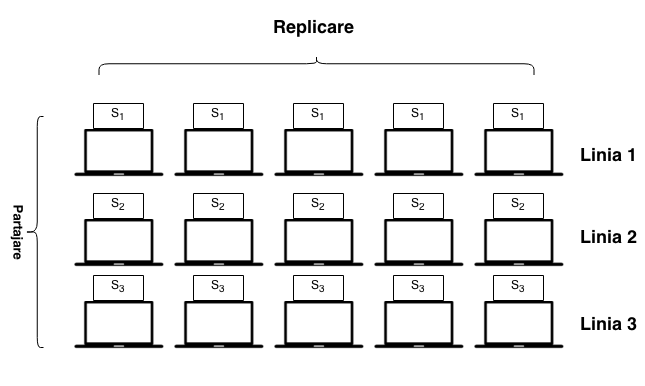
\includegraphics[width=12cm]{img/GridSharing.png}    % The printed column width is 8.4 cm.
	\caption{GridSharing cu $3$ linii, $15$ servere dintre care $2$ bizantine, $1$ cu scurgeri de informa\c{t}ii \todo{citare}}
	\label{fig:grid_sharing}
	\bigskip
\end{figure}


\subsection{POTSHARDS} 
\label{sec:desc_potshards}
\^{I}n $2007$ este propus un nou sistem care combin\u{a} caracteristicile PASIS \c{s}i GridSharing ad\u{a}ug\^{a}nd posiblitatea de migrarea a datelor la noduri noi: POTSHARDS \todo{(Protection Over Time, Securely Harboring
And Reliably Distributing Stuff)) - mereu prima data cand folosesti o abreviere trebuie sa o explici}

\todo{cite! se citeaza la inceput}

De asemenea este introdus\u{a} o tehnic\u{a} nou\u{a} de g\u{a}sire a componentelor folosind pointeri aproximativi. Pentru a asigura confiden\c{t}ialitatea, autorii adopt\u{a} o schem\u{a} de partajare XOR unanim\u{a}, la fel ca \^{i}n GridSharing.
POTSHARDS consider\u{a} problema \^{i}n care o persoan\u{a} neautorizat\u{a} \^{i}ncearca s\u{a} afle informa\c{t}ii vulnerabile f\u{a}r\u{a} ca aceasta sa fie nedetectat\u{a}. Schemele existente precum PASIS \c{s}i GridSharing nu indeplineau aceast\u{a} cerin\c{t}a dac\u{a} un atacator determin\u{a} loca\c{t}ia componentelor distribuite ini\c{t}ial.
\todo{nu inteleg - reformulare, explica ce vrei sa zici!}

Solu\c{t}ia pe care o ofer\u{a} aceast\u{a} arhitectur\u{a} este reconstruirea componentelor \^{i}ntr-un mod securizat si folosirea semn\u{a}turilor algebrice pentru a asigura un grad ridicat de p\u{a}strare a integrita\c{t}ii fi\c{s}ierelor \cite{STM:2006}.
POTSHARDS poate fi g\^{a}ndit ca o aplica\c{t}ie pe partea clientului care comunic\u{a} cu o mul\c{t}ime de noduri (arhive) independente.

Ca prim pas, POTSHARDS preproceseaz\u{a} fi\c{s}ierul \^{i}ntr-un obiect, partajeaz\u{a} obiectul \^{i}n fragmente la care adaug\u{a} meta-date, numite \textit{shards} (Fig. \ref{fig:data-potshard}) \cite{SGMV:2009}. Acestea sunt trimise apoi arhivelor independente, fiecare av\^{a}nd propriul domeniu de securitate, localizate in \textit{regiuni}. Pentru a reconstitui cu succes informa\c{t}ia ini\c{t}iala, meta-datele shard-urilor con\c{t}in detalii despre structura pointerilor aproximativi, indic\^{a}nd regiunea \^{i}n care se afl\u{a} urm\u{a}torul shard.

\begin{figure}
	\begin{center}
	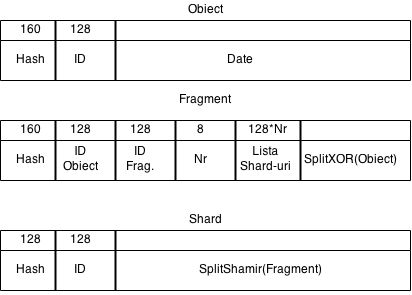
\includegraphics[width=7cm, height=4cm]{img/Shards.png}    % The printed column width is 8.4 cm.
	\caption{Entit\u{a}\c{t}i de date in POTSHARDS. $Nr$ e num\u{a}rul de shard-uri produse de un fragment.
		$SplitXOR$ reprezint\u{a} o component\u{a} rezultat\u{a} \^{i}n urma partajarii unanime XOR. Analog $SplitShamir$ reprezint\u{a} o component\u{a} rezultat\u{a} \^{i}n urma partajarii folosind schema Shamir. \todo{cite!}}
	\label{fig:data-potshard}
	\bigskip
	\end{center}
\end{figure}

Procesul de fragmentare a datelor este prezentat in Fig. \ref{fig:potshards-layers}.

\begin{figure}
	\begin{center}
	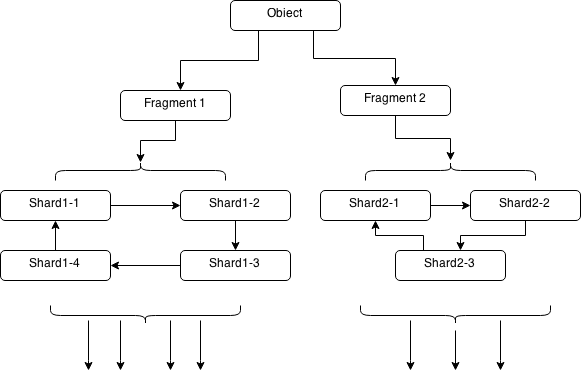
\includegraphics[width=12cm]{img/POTSHARDS.png}    % The printed column width is 8.4 cm.
	\caption{Distribuirea unui obiect in POTSHARDS}
	\label{fig:potshards-layers}
	\bigskip
	\end{center}
\end{figure}

Pentru ca reconstituirea unui fi\c{s}ier sa fie fezabil\u{a} unui utilizator, acestuia \^{i}i este \^{i}ntoars\u{a} o list\u{a} cu loca\c{t}iile exacte shard-urilor corespunz\u{a}toare.
Ob\c{t}inerea unui shard de c\u{a}tre un atacator nu este folositoare, pentru a detecta urm\u{a}torul shard, un atac brut force const\u{a} \^{i}n cereri multiple \^{i}n zona indicat\u{a} de pointerul aproximativ. Un astfel de atac nu va trece neobservat de POTSHARDS deorece unul dintre scopurile sale este s\u{a} stocheze datele \^{i}ntr-un mod cat mai uniform distribuit \todo{spread}.\cite{SGMV:2009}

\section{Alouneh et al.}
\todo{Alt nume poate?}
\label{sec:desc_alouneh}
Autorii propun un sistem pentru stocarea datelor un timp indelungat folosind schema Shamir cu c\^{a}teva modific\u{a}ri. Aceste schimb\^{a}ri se vor ar\u{a}ta cruciale mai t\^{a}rziu \^{i}n men\c{t}inerea securit\u{a}\c{t}ii.

\subsection{Arhitectura sistemului}

\^{I}n cazul \^{i}n care dorim sa stoc\u{a}m un fi\c{s}ier \^{i}n sistem (abord\^{a}nd filozofia majorit\u{a}\c{t}ii sistemelor de operare - orice este un fi\c{s}ier), acesta este preluat de o aplica\c{t}ie de control pe partea de client pe care \^{i}l \^{i}mparte \^{i}n blocuri de octe\c{t}i de lungime $k$. Pentru fiecare bloc, octe\c{t}ii devin coeficien\c{t}ii unui polinom $f$, componenta cu indicele $i$ va fi reprezentat\u{a} de valoarea lui $f(i)$ $i = \{1,2,\dots, n\}$. Men\c{t}ion\u{a}m c\u{a} toate opera\c{t}iile se vor efectua in $GF(256)$ modulo un polinom ireductibil (\^{i}n implementarea sistemului, autorii folosesc $x^8 + x^5 + x^3 + x + 1$). Procedeul este descris in detaliu in Fig \ref{fig:alouneh_distribution}.


%---------------- Figure - alouneh-distribution - START ------------------------
\begin{figure*}[h!]

\begin{tabular}{|p{\textwidth}|}
\hline

\\
\hspace{.1in}
\textbf{Date de intrare}: Un fi\c{s}ier binar $\mathcal{S}$;
\medskip

\hspace{.1in}
\textbf{Date de ie\c{s}ire}: $n$ fi\c{s}iere binare distribuite la noduri din re\c{t}ea;
\medskip

\hspace{.1in}
\textbf{Procesarea componentelor}: Aplica\c{t}ia existent\u{a} pe partea clientului: 
	\begin{itemize}
		\item Dac\u{a} $\mathcal{S}$ nu are o lungime divizibil\u{a} cu $k$:
			\begin{itemize}
			\item Concateneaz\u{a} la sf\^{a}rsitul lui $\mathcal{S}$ octe\c{t}i p\^{a}n\u{a} c\^{a}nd $len(\mathcal{S}) \Mod k = 0$;
			\end{itemize}
		\item \^{I}mparte $\mathcal{S}$ \^{i}n blocuri de lungime $k$;
		\item Repet\u{a} pentru fiecare bloc $B_t$ de lungime $k$:
		\begin{itemize}
			\item Construie\c{s}te polinomul $f(x) = B_{t_{k - 1}}x ^ {k-1} + B_{t_{k - 2}}x ^ {k - 2} + .... + B_{t_1}x + B_{t_0}$;
			\item Calculeaz\u{a} $f(i)$ pentru $1 \leq i \leq n$;
		\end{itemize}
	\end{itemize}

\hspace{.1in}
\textbf{Distribu\c{t}ie}: Aplica\c{t}ia la nivelul clientului:
	\begin{itemize}
		\item Distribuie componenta $f(i)$ nodului din re\c{t}ea cu indicele $i$:
	\end{itemize}

\\
\hline
\end{tabular}
\caption{Schema Alouneh et al. - Generare \cite{AAMK:2013}}
\label{fig:alouneh_distribution}
\end{figure*}

%---------------- Figure - alouneh_distribution - STOP ------------------------

\begin{example}
Vom exemplifica modul de calcul \^{i}n $GF(256) \Mod {g(x)} $ unde $g(x) = x ^ 8 + x ^ 4 + x ^ 3 + 1$. Lu\u{a}m polinomul $f(x) = 10 + 15x$ care corespunde unui fi\c{s}ier format din octe\c{t}ii (\^{i}n aceast\u{a} ordine) $10$ $15$.
	\begin{equation} \label{eq:f_01}
	\begin{split}
		f(01) \Mod{g(x)} & = 10 + 15 \Mod{g(x)} \\
		& = (x ^ 4) + (x ^ 4 + x ^ 2 + 1) \Mod{g(x)} \\
		& = x ^ 2 + 1 = 000000101_2 \\
		& =  05_{16}
	\end{split}
	\end{equation}

	\begin{equation} \label{eq:f_02}
	\begin{split}
	 f(02) \Mod{g(x)} & = 10 + 15\cdot02 \Mod{g(x)} \\
	 & = (x ^ 4) + (x ^ 5 + x ^ 3 + x) \Mod{g(x)} \\
	 & = 00111010_2 \\
	 & = 3A_{16}
	 \end{split}
	 \end{equation}
\end{example}
Pentru reconstituirea unui fi\c{s}ier (\ref{fig:alouneh_reconstruction}) se interpoleaz\u{a} din orice mul\c{t}ime de componente $A$ cu dimensiune minim $k$ prin metoda lui Lagrange, asem\u{a}n\u{a}tor schemei Shamir:
\begin{equation}
	\label{eq:lagrange_poly}
	f(x)=\sum_{i \in A} f(i) \prod_{j \in A, j \neq i} \frac{x-j}{i-j}
\end{equation}

\begin{example}
Vom exemplifica interpolarea \ref{eq:lagrange_poly} pe componentele calculate in  \ref{eq:f_01} si \ref{eq:f_02} pentru a reconstitui polinomul:
	\begin{equation}
	\begin{split}
		f(x) & = 05(x - 02)(01 - 02)^{-1} + 3A(x - 01)(02 - 01)^{-1} \\
		& = 05(x - 02)03^{-1} + 3A(x - 01)03^{-1} \\
		& = F6(05 + 3A)x + F6(05\cdot02 + 3A \cdot 01) \\
		& = F6\cdot 3F\cdot x + F6\cdot30 = 15x + 10
	\end{split}
	\end{equation}
\end{example}

Noutatea arhitecturii const\u{a} in diminuarea redundan\c{t}ei componentelor la un factor de $k$, spre deosebire de sistemele descrise in \ref{sec:desc_pasis} sau in \ref{sec:desc_potshards}. Reducerea spa\c{t}iului ocupat este datorat \^{i}nlocuirii coeficien\c{t}ilor cu octe\c{t}ii din fi\c{s}ierul ce va fi partajat. Confiden\c{t}ialitatea este indus\u{a} \^{i}n mod automat de schema lui Shamir.

%---------------- Figure - alouneh-reconstruction- START ------------------------
\begin{figure*}[h!]

\begin{tabular}{|p{\textwidth}|}
\hline

\\
\hspace{.1in}
\textbf{Date de intrare}: Cel pu\c{t}in $k$ componente provenite din noduri (distincte);
\medskip

\hspace{.1in}
\textbf{Date de ie\c{s}ire}: Fi\c{s}ierul binar original $\mathcal{S}$;
\medskip

\hspace{.1in}
\textbf{Reconstruc\c{t}ie}: Aplica\c{t}ia existenta pe partea clientului: 
	\begin{itemize}
		\item Repet\u{a} pentru fiecare bloc al lui $\mathcal{S}$:
		\begin{itemize}
			\item Calculeaz\u{a} prin interpolare coeficien\c{t}ii lui $f(x)=B_{t_{k - 1}}x ^ {k-1} + B_{t_{k - 2}}x ^ {k - 2} + .... + B_{t_1} + B_{t_0}$
			\item Reconstituie blocul $B_t$
		\end{itemize}
		\item \c{S}terge octe\c{t}ii de la sf\^{a}r\c{s}itul fi\c{s}ierului ad\u{a}uga\c{t}i la generare. 
	\end{itemize}

\\
\hline
\end{tabular}
\caption{Schema Alouneh et al. - Reconstruc\c{t}ie \cite{AAMK:2013}}
\label{fig:alouneh_reconstruction}
\end{figure*}

%---------------- Figure - alouneh_reconstruction- STOP ------------------------
%TODO: add reconstruction and pictures with different architectures, maybe some examples.
%----------------------------------------------------------------
%----------------------------------------------------------------
%----------------------------------------------------------------
%----------------------------------------------------------------
%----------------------------------------------------------------
\section{Rezultate obtinute}
Impreuna cu mentorul am analizat un articol aparut intr-un jurnal de clasa C, prezentat in (\ref{sec:desc_alouneh}) unde am indentificat erori majore ale sale si am implementat sistemul descris de autori pentru a demonstra practic, nu doar teoretic anumite greseli pe care le vom evidentia in urmatoarele sectiuni. \cite{AAMK:2013}

\label{sec:results}
\subsection{Erori gasite in articol}

Spre deosebire de schema Shamir, unde coeficientii sunt alesi intr-un mod aleator uniform, acestia sunt extrasi din continutul fisierelor originale.
Alegerea este motivata de faptul ca multimea componentelor si efortul computational depus pentru generarea coeficientilor se reduce la un factor de $k$ spre deosebire de schema Shamir.

Natura determinismului duce la cateva atacuri simple in momentul in care un atacator obtine informatiile stocate intr-un nod, indiferent de marimea pragului folosit in metoda de partajare. Datorita acestuia, am aratat 2 atacuri simple in cazul in care componentele sunt calculate in ordine:
\begin{itemize}
	\item Detectarea tipului unui fisier
	\item Detectarea tipului de continut unui fisier
\end{itemize}

Am indicat ca un atac bazat pe felul in care se realizeaza completarea fisierului $\mathcal{S}$ inainte de partajarea sa poate fi fezabil, in conditiile in care s-a demonstrat ca aceasta alegere este esentiala in pastrarea securitatii \cite{Vaudenay:2002}.

\subsubsection{Detectarea tipului de fisier}\hspace*{\fill} \\
\label{subsec:file_type_detection}

In sistemele de operare, la inceputul fiecarui fisier se afla o secventa de octe\c{t}i (semnatura sau antet) pentru a determina tipul acestuia. In tabelul (\ref{table:sign}) gasim 4 din cele mai uzuale antete.

Considerand cazul in care dorim sa partajam un fi\c{s}ier \textit{pdf} cu ajutorul sistemului descris in \ref{sec:desc_alouneh} folosind $k \leq 4$. Polinomul corespunzator $f(x)$ va fi intotdeauna acela\c{s}i. Presupn\^{a}nd ca numerotarea nodului $i$ este aceeasi, putem determina cu usurinta daca este stocat un fisier \textit{pdf} fara a lua in vedere continutul fisierului.

Cu alte cuvinte, daca un adversar obtine controlul unui singur nod, bazandu-se doar pe valoarea primei componente poate detecta tipul unui fisier.

In plus, pastrand aceeasi presupunere, anume ca nodurile isi pastreaza acelasi indice $i$ iar adversarul obtine valorile $i$ si $k$ atunci acesta poate detecta cu o probabilite ridicata tipul fisierului folosindu-se de prima componenta. Ne asumam posibilitatea datorita faptului ca valoarea lui $k$ este publica iar $i$ poate sa fie descoperita la distribuire (Fig. \ref{fig:alouneh_distribution}).

Pentru a exemplifica, un adversar poate distinge cu probabilitate ridicata intre fisierele \textit{doc, gif, pdf, png, rar, wav} si \textit{zip}. In tabelul (\ref{table:shares}) avem generate componentele pentru $k = 2$ si $n = 5$.
Daca un adversar descopera ca valoarea primului nod este $14$ atunci acesta afla ca pentru prima componenta corespunde un fisier \textit{gif}. Daca obtine accesul nodului $4$ si citeste valoarea $205$ atunci stie ca fisierul este de tipul \textit{rar}. Daca citeste valoarea $27$ de pe primul nod atunci stie ca poate fi un \textit{wav} sau \textit{zip}. Cu toate acestea poate sa distinga cele 2 fisiere daca dezvaluie o singura valoare de pe celelalte noduri ($2 3 4 5$) pentru ca valorile sunt distincte.

%-----------------------------------------------------
\begin{table}
\begin{center}
\caption{Semnaturi de fisiere}\label{tb:margins}
\label{table:sign}
\begin{tabular}{ccccc}
Tip de fi\c{s}ier &  \multicolumn{4}{c}{Primii 4 octe\c{t}i}\\ \hline 
doc &  D0 & CF & 11 & E0\\
gif & 47 & 49 & 46 & 38 \\
pdf & 25 & 50 & 44 & 46 \\
png & 89 & 50 & 4E & 47 \\
rar & 52 & 61 & 72 & 21 \\
wav & 52 & 49 & 46 & 46 \\
zip & 50 & 4B & 03 & 04\\  \hline
\end{tabular}
\end{center}
\bigskip
\end{table}

%-----------------------------------------------------
\bigskip
\begin{table}
\begin{center}
\caption{Componentele primului bloc ($k=2$)}\label{tb:margins}
\label{table:shares}
\begin{tabular}{cccccccc}
Tip fisier & Nod 1 & Nod 2 & Nod 3 & Nod 4 & Nod 5 \\
  & ($i=1$) & ($i=2$) & ($i=3$) & ($i=4$) & ($i=5$) \\
\hline
doc & 31 & 85 & 154 & 193 & 14 \\
gif & 14 & 213 & 156 & 120 & 49 \\
pdf & 117 & 133 & 213 & 126 & 46 \\
png & 217 & 41 & 121 & 210 & 130 \\ 
rar & 51 & 144 & 241 & 205 & 172  \\
wav & 27 & 192 & 137 & 109 & 36 \\
zip & 27 & 198 & 141 & 103 & 44 \\ \hline
\end{tabular}
\end{center}
\bigskip
\end{table}

%-----------------------------------------------------

\subsubsection{Detectarea tipului de con\c{t}inut}\hspace*{\fill} \\
\label{subsec:file_content_detection}

Multe documente urmeaza un anumit tipar precum contracte, chitante, bonuri fiscale sau curriculum vitae. Deoarece majoritatea continutului ramane neschimbat, exista o probabilitate destul de mare ca multe componente sa aiba aceeasi valoare. O data ce un adversar reuseste sa determine compontentele unui nod, poate determina prin analogie tipul de continut al fisierului original.

Fisierele cele mai vulnerabile sunt cele care contin o secventa de octeti periodica (imagini cu un pattern repetitiv) sau cele care multi octeti nuli(valoarea componentelor va fi $0$).


\subsection{Verificarea rezultatelor}
Pentru a arata aplicabilitatea rezultatelor in practica, am implementat propunerea descrisa in sectiunea {\ref{sec:desc_alouneh}} si am testat pe cateva cazuri.

In cadrul implementarii am folosit limbajul Python3.0 in cadrul sistemului de operare ArchLinux.

Python este un limbaj de programare cu tipuri dinamice, disponibil sub licenta open-source \cite{Python:2015}. Pentru a realiza comunicarea intre procese am folosit Cerealizer iar distributia componentelor a fost vizual generata cu ajutorul pachetului Matplotlib \cite{Hunter:2007, PyCerealizer:2015}. De asemenea am folosit sistemul de versionare Git iar codul e gazduit de GitHub \cite{Github:2015, CodeGit:2015}.

Avand in vedere ca articolul original nu mentioneaza o metoda de padding, am considerat o metoda standard pentru a completa octetii ultimului bloc: alipim la sfarsitul lui $\mathcal{S}$ octetii $80$ $00$ $00$ $\dots$ $00$ $00$ pana cand lungimea ultimului bloc ajunge la $k$ octeti.

Mentionam aceasta metoda doar pentru completitudine, aceasta neafectand rezultatele, considerand doar secventele de octeti de la inceputul fisierului sau antentul s\u{a}u.

\subsubsection{Detectarea tipului de fi\c{s}ier}\hspace*{\fill} \\

Extindem analiza facuta in sec\c{t}iunea {\ref{subsec:file_type_detection}} asupra tipurilor din tabelul {\ref{table:sign}} pentru $k = 2$ si crestem valoarea indicelui $i$ pana cand 2 componente devin egale. Fie $f_l$ polinomul de gradul $1$ asociat primului bloc al fisierului aflat pe linia $l$. Analog $f_c$ polinomul de gradul $1$ asociat primului bloc al fisierului aflat pe coloana $c$.

In tabelul {\ref{table:k2}} calculam valoarea maxima a nodului $i$ pentru care $f_l(i) \neq f_c(i)$. Valoarea $-1$ indica lipsa de coliziuni ale lui $f_c(x)$, $f_l(x)$ pentru $i$, $i = {1,2,\dots,255}$ ($\not\exists 1 \leq i \leq 255$ a.\^{i}. $f_l(i) = f_c(i)$)).

Deoarece pe diagonala principala toata componentele sunt identice pentru $k <= 4$ poate fi ignorata. In tabelul {\ref{table:k2}} observam valoarea $0$ pentru perechea $(wav, zip)$ pentru ca $f_wav(1) = f_zip(1) = 27$ (tabel \ref{table:sign}).

In tabelele {\ref{table:k3}, \ref{table:k4}} sunt considerate rezultatele pentru $k = 3$ si $k = 4$. Pentru $k \geq 5$ este nevoie de un antet cu mai mult de $4$ octeti.


%-----------------------------------------------------
\begin{table}[b]
\bigskip
\begin{center}
\caption{Indicele maxim $i$ a.\^{i} componentele primului bloc sa fie distincte($k=2$)}\label{tb:margins}
\label{table:k2}
\begin{tabular}{cccccccc}
Tip Fi\c{s}ier & doc & gif & pdf & png & rar & wav & zip \\\hline
  doc & - & 169 & 194 & 209 & 170 & 206 & 110\\
  gif & 169 & - & 133 & 137 & 75 & -1 & 133\\
  pdf & 194 & 133 & - & -1 & 115 & 151 & 133\\
  png & 209 & 137 & -1 & - & 229 & 147 & 195\\
  rar & 170 & 75 & 115 & 229 & - & -1 & 42\\
  wav & 206 & -1 & 151 & 147 & -1 & - & 0\\
  zip & 110 & 133 & 133 & 195 & 42 & 0 & -\\ \hline
\end{tabular}
\end{center}
\bigskip
\end{table}




%-----------------------------------------------------

\begin{table}
\begin{center}
\caption{Indicele maxim $i$ a.\^{i} componentele primului bloc sa fie distincte($k=3$)}\label{tb:margins}
\label{table:k3}
\begin{tabular}{cccccccc}
Tip Fi\c{s}ier & doc & gif & pdf & png & rar & wav & zip \\\hline
  doc & - & 63 & -1 & -1 & -1 & -1 & -1\\
  gif & 63 & - & -1 & -1 & -1 & -1 & -1\\
  pdf & -1 & -1 & - & 164 & -1 & 119 & -1\\
  png & -1 & -1 & 164 & - & 143 & 122 & 129\\
  rar & -1 & -1 & -1 & 143 & - & 143 & -1\\
  wav & -1 & -1 & 119 & 122 & 143 & - & 172\\
  zip & -1 & -1 & -1 & 129 & -1 & 172 & -\\ \hline
\end{tabular}
\end{center}
\bigskip
\end{table}

%-----------------------------------------------------
\begin{table}
\begin{center}
\caption{Indicele maxim $i$ a.\^{i} componentele primului bloc sa fie distincte($k=4$)}\label{tb:margins}
\label{table:k4}
\begin{tabular}{cccccccc}
Tip Fi\c{s}ier & doc & gif & pdf & png & rar & wav & zip \\\hline
  doc & - & -1 & 38 & 95 & 1 & 95 & 98\\
  gif & -1 & - & -1 & -1 & 167 & -1 & -1\\
  pdf & 38 & -1 & - & 12 & 11 & 119 & 70\\
  png & 95 & -1 & 12 & - & 243 & 95 & 148\\
  rar & 1 & 167 & 11 & 243 & - & -1 & 94\\
  wav & 95 & -1 & 119 & 95 & -1 & - & -1\\
  zip & 98 & -1 & 70 & 148 & 94 & -1 & -\\ \hline
\end{tabular}
\end{center}
\bigskip
\end{table}




%-----------------------------------------------------

\subsection{Publicarea articolului}

%
% ---- Bibliography ----
%
%\begin{thebibliography}{5}
%
\bibliographystyle{splncs}
\bibliography{llncs}

%\end{thebibliography}

\end{document}
